\subsection{AI-Assisted Framework Overview}

The development of ecosystem models requires substantial time organizing species into functional groups and determining their interactions. This framework automates these tasks through a five-stage process that integrates artificial intelligence with ecological databases (Figure~\ref{fig:framework_overview}).

The first step in the process is to define a model domain and the resultant shapefile is used to derive a comprehensive species list from Ocean Biodiversity Information System (OBIS) \citep{Grassle1999}. In Stage 2, this species list is enriched with ecological data from FishBase and SeaLifeBase \citep{froese2010fishbase}, which provide life history traits, ecological parameters, and diet information, and with trophic interactions from the Global Biotic Interactions (GLOBI) database \citep{Poelen2014}.

Stage 3 employs a LLM for species grouping. We use Claude Sonnet-3.5 (hereafter referred to as `Claude')\citep{Anthropic2024}, though other LLMs can be incorporated. The grouping process considers both the research focus specified by the user and a generic grouping template, assigning species into functional groups.

\begin{figure}[htbp]
    \centering
    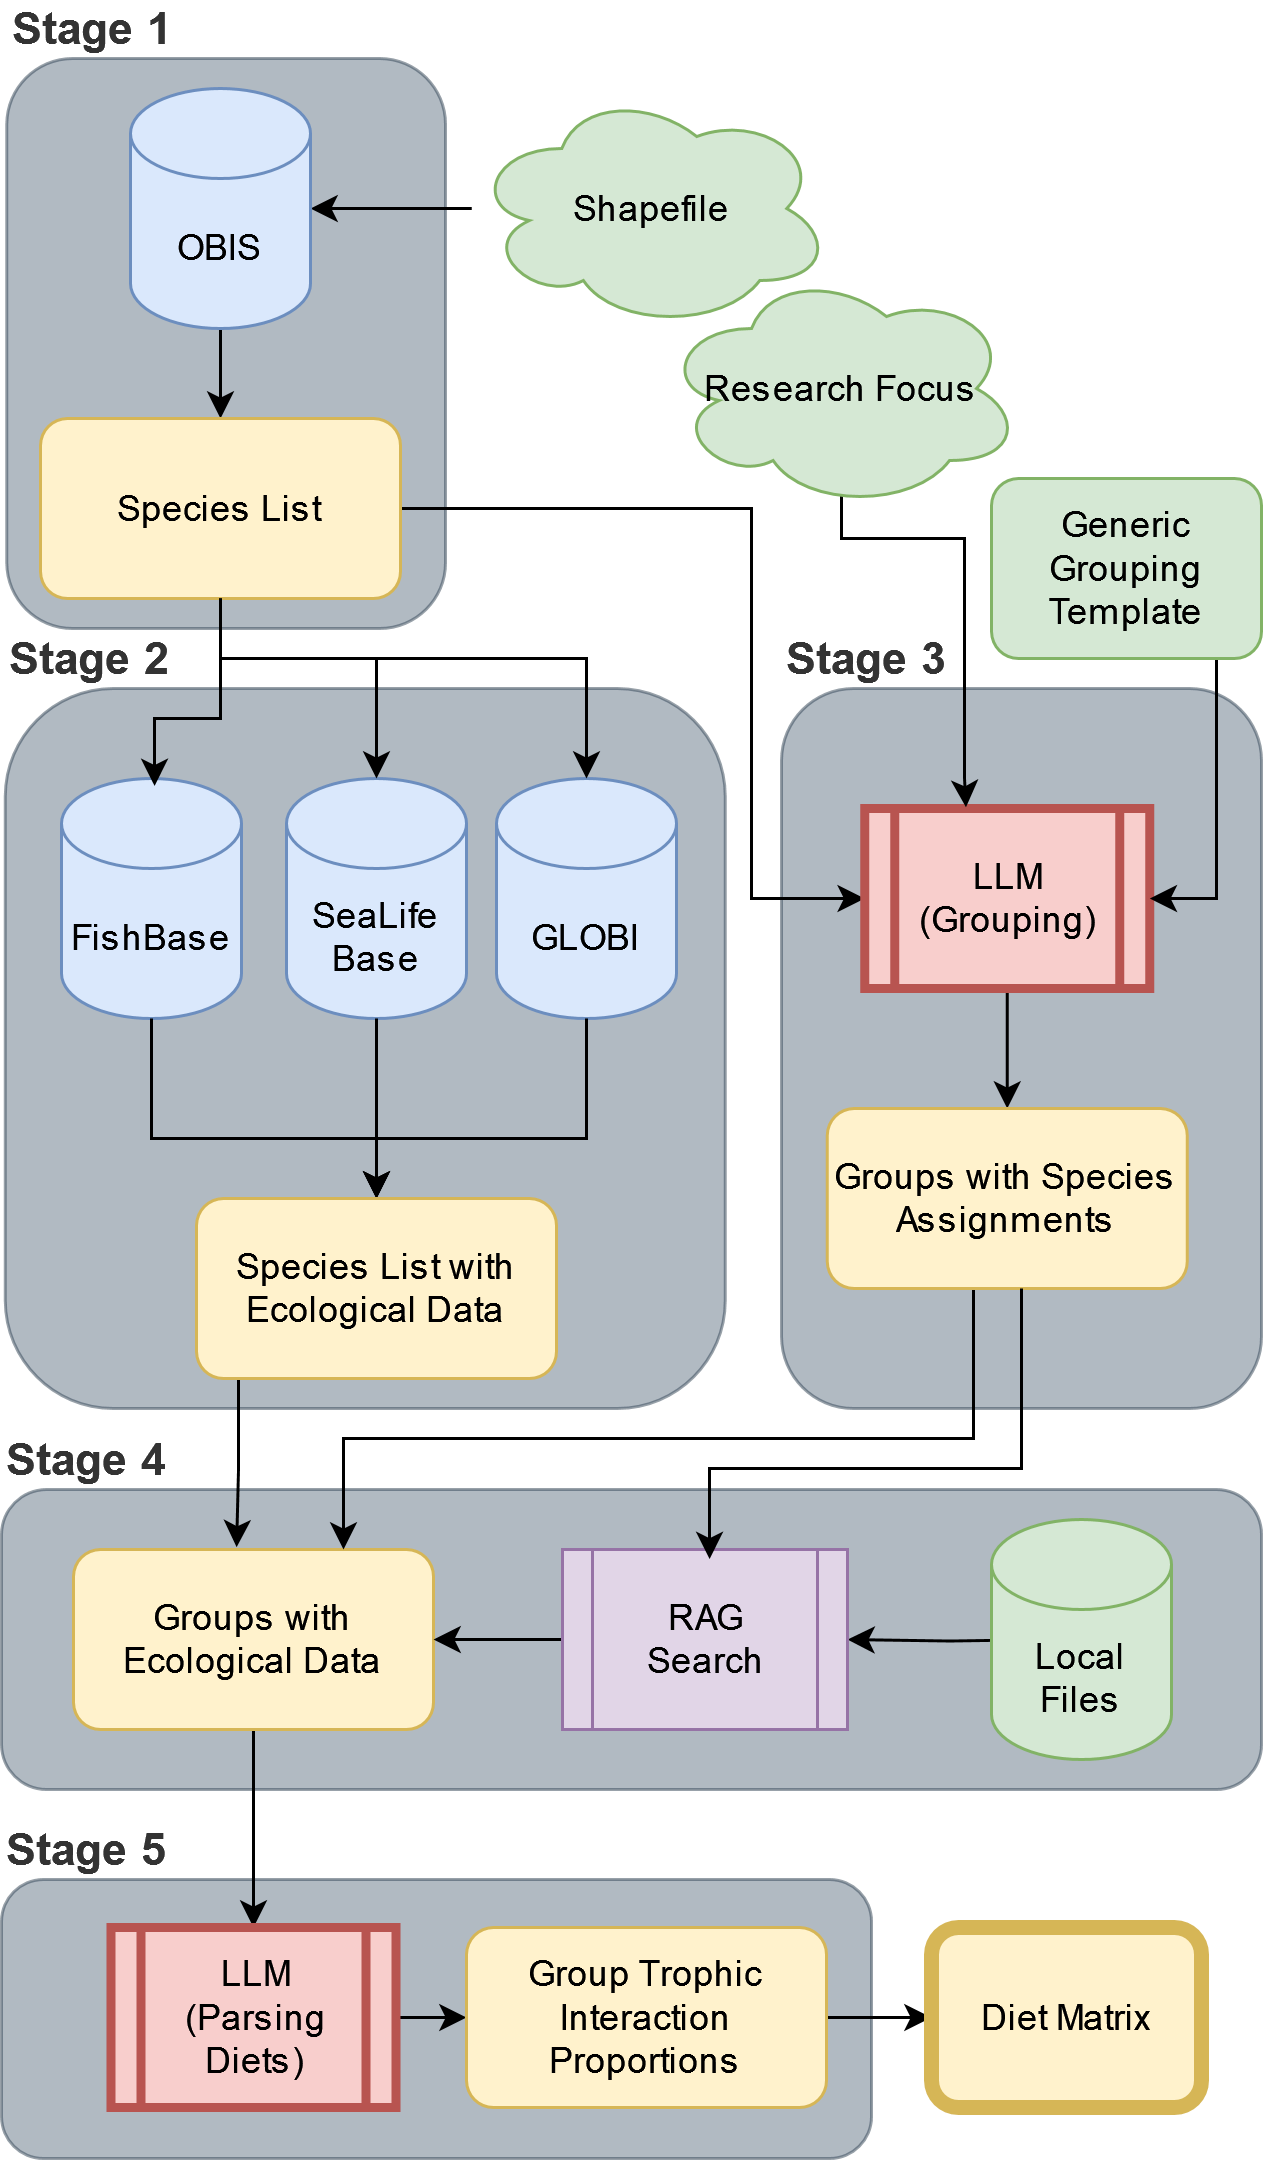
\includegraphics[width=0.5\textwidth]{figures/EwE_AI.drawio.png}
    \caption{Overview of the AI-assisted framework for ecosystem model development. The process consists of five stages: species identification, ecological data collection, functional group organization, diet data synthesis, and diet matrix construction. Each stage integrates multiple data sources and analytical approaches, with user-provided inputs (shown in green) guiding key decisions.}
    \label{fig:framework_overview}
\end{figure}

Stage 4 uses a retrieval augmented generation (RAG) system (e.g. \citep{keck2025extracting}) to synthesize the species-level ecological data into group-level summaries and incorporates user-provided local knowledge from a vector storage database (a database that stores and retrieves information based on semantic similarity rather than exact text string matching), Chroma \citep{Chroma2024}, to produce group-level diet composition estimates. Finally, Stage 5 uses the LLM to parse and structure this combined data into a diet matrix, determining trophic interaction proportions among functional groups.

Section~\ref{supp:4} of the supplementary material contains detailed documentation of all processing steps, including database queries, literature search criteria, and ecological classification rules. The complete codebase and configuration files reside at [GitHub repository URL, removed for peer-review].
